\chapter{Monitoring neuronal activity over days during learning blah} \label{chapter_4}

\section{Introduction}\label{sec:chap4_intro}

Given that changing neuronal activity patterns either cause some instability in information coding or require compensation by a dynamic decoding network, it is important to consider what advantages might arise from these changes. Computational models suggest that an advantage of dynamic neuronal representations could be the flexibility of incorporating new information into the population (Ajemian et al., 2013; Rokni et al., 2007). 

\section{Results} \label{sec:chap4_results}

\subsection{Task Design for Learning a Stimulus-Action Pair} \label{chap4:stim_action}

We therefore tested how existing representations were affected by the learning of a new association. We trained the same mice that had already stably performed the task described above to learn a new association. We introduced a third possible cue (crosshatch pattern) that required a specific turn at the intersection for the mouse to receive a reward (the turn direction was randomly selected for each mouse) (Figure 7A). After a mouse had learned the novel third trial type, we introduced a fourth cue (triangle pattern) that required the mouse to turn the opposite direction of that required for the third cue (Figure 7A). Mice learned the novel cue-response associations while maintaining high performance for the original two cue-response associations (Figure 7B).

\subsection{Decoding Trial Type Information Over the Course of Learning} \label{chap4:decoding}

We first asked whether the neuronal activity patterns were different between trials in which the mouse saw the novel cues and those in which it saw the familiar cues. Using a decoder based on population activity, the novel trial types were separable from the familiar trial types (Figure 7C). These differences in activity between trial types could be visualized on a single day based on population activity in a dimensionality-reduced space (Figure 7D). We tested if the addition of new learned associations altered the rate at which neuronal activity patterns changed during performance of previously learned trial types. We might expect learning to increase the rate of change as new information is incorporated into network activity. Surprisingly, we found that the rate of change was comparable between the days with stable performance of the two familiar trial types and during learning of the novel trial types (measured based on the performance of models of cells'�� activity-behavior relationships across days, as in Figure 4C-E) (Figure 7E-F).

\subsection{Rate of Change During Learning Compared to Stable Behavior} \label{chap4:rate_change}

This similar rate of change could have occurred because the cells with activity related to the novel trial types were different from the cells with activity related to familiar trial types. We therefore analyzed if the cells with activity related to novel cues had activity related to familiar cues on previous days. Surprisingly, cells with activity related to novel cues were more likely to come from the group of cells which recently (within the past ten days) had activity related to the familiar cues than from a random sample of neurons (Figure 7G-H). 
\begin{figure}

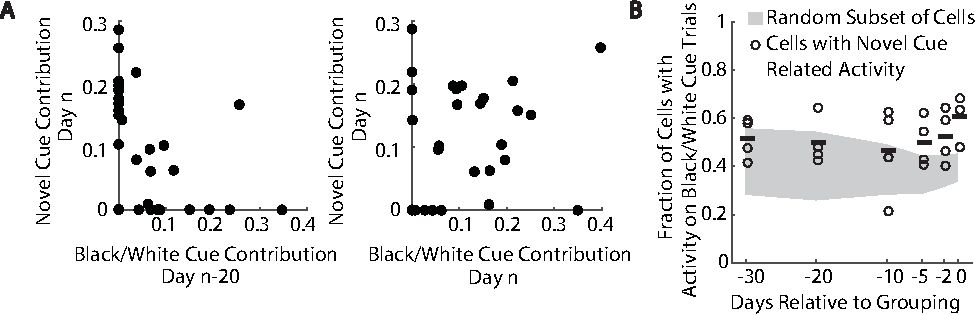
\includegraphics[width=\textwidth]{figures/7_learning_same_pool.pdf}
\caption[Behavioral training procedure for the fixed association evidence accumulation task]{\textbf{Behavioral training procedure for the fixed association evidence accumulation task. a,}
Sequence of mazes used for behavioral training. Asterisks indicate reward location. Only some example mazes are shown (for example, right choice and not left choice maze in maze 1).
%
\textbf{b,} Distribution of net evidence corresponding to different difficulties used in training the final task (maze 8; see \textbf{d}).
%
\textbf{c,} Screen captures of the virtual environment at cue 1, cue 6, and the turn in maze 8.
%
\textbf{d,} Behavioral performance across sessions for three example mice. Colors correspond to the maze colors indicated in \textbf{a}. Shapes correspond to the net evidence probabilities in \textbf{b}.
\label{figures/7_learning_same_pool}}
\end{figure}


The evolving pool of cells involved in representing task features was thus more likely to incorporate new task relevant information than the group of cells presently without task relevant information. This finding suggests that new information can be incorporated into the pool of task relevant activity as this pool continuously shifts over time, without disrupting baseline functionality. We speculate that the ability to incorporate new information using 'multitasking' neurons could allow for flexibility during learning, such that the network's ongoing changes provide a framework for the addition of new associations.

\section{Methods} \label{sec:chap4_methods}

Training for novel trial type associations was performed during imaging. Mazes were identical to maze 5. On each day, mice were presented with novel trial types after 40 trials of the original trial types (black cue-right turn and white cue-left turn). After novel trial types were introduced, familiar trial types and novel trial types were interleaved such that there were equal fractions of left and right turn trials. Mice were first presented with a 3rd cue (crosshatch) and after mice performed all three trial types at above 80 $\%$ for three consecutive days, we introduced a 4th cue (triangles). For mouse 1, the 3rd cue instructed left turns and the 4th cue instructed right turns. For mouse 2, the cue-turn relationship for novel trial types was reversed. White and black cues maintained consistent cue-turn relationships for both mice. Mice learned novel trial type cue-turn relationships by trial and error while maintaining previously learned relationships for black and white cues. 

\section{Discussion} \label{sec:chap4_discussion}

We speculate that the changes in neuronal activity reported here reveal key features of how associations are formed and represented in PPC. In particular, our work reveals a potential strategy for a population of neurons to achieve stability in the maintenance of learned associations while also allowing flexibility to incorporate new information. 